	\section{Computational experiments}\label{section:experiments}
This section is devoted to studying the performance of \eqref{form:H-TSPHN} and \eqref{form:H-TSPN} formulations proposed in Section \ref{section:formulations}. In the first subsection, the procedure for generating the considered random instances is described. The second subsection details the experiments that have been conducted. The third subsection reports the results obtained in these experiments.

\subsection{Data generation}
%To generate the instances of our experiments, it is necessary that these instances verify the assumptions \ref{A1}-\ref{A4} stated in the Section \ref{section:description}. 

To generate the instances of our experiments, we assume  assumptions \ref{A1}-\ref{A4} stated in Section \ref{section:description}. The following proposition gives an upper bound for the number of balls that can be generated given an instance with $n=|\mathcal B|$ barriers:

%		\JP{	
	%		\begin{prop}
		%			Under the hypothesis that balls are \CV{not} visible among them, the maximum number of balls that can be considered in \TSPHN \ is $O(n^2)$.
		%		\end{prop}
	%		\begin{proof}
		%			The proof is based on the properties of the visibility graph $VG(\cal B)$ of the configuration of barriers in $\cal B$:  It is clear that the maximum number of balls coincides with the number of faces, $f_{VG(\cal B)}$, of $VG(\cal B)$.  Recall that the number of vertices in $\cal B$ is $n$. Next, by the Euler formula, the number of faces $f_{VG(\cal B)}$ is $2+E_{VG(\cal B)}-n$. Since $E_{VG(\cal B)}=O(n^2)$, it follows that $f_{VG(\cal B)}=O(n^2)$.
		%		\end{proof}
	%	}


\begin{prop}
	Under assumptions \ref{A1}-\ref{A4}, the maximum number of balls that can be considered in \TSPHN \ is $O(n^2)$.
\end{prop}
\begin{proof}
	The proof is based on the properties of the visibility graph $VG(\cal B)$ of the configuration of barriers in $\cal B$ \citep{mitchell_shortest_2017}:  It is clear that the maximum number of balls coincides with the number of faces, $f_{VG(\cal B)}$, of $VG(\cal B)$.  Recall that the number of vertices in $\cal B$ is $n$. Next, by the Euler formula the number of faces $f_{VG(\cal B)}$ is $2+E_{VG(\cal B)}-n$. Since $E_{VG(\cal B)}=O(n^2)$, it follows that $f_{VG(\cal B)}=O(n^2)$.
\end{proof}


The idea is to generate line segments located in general position without crossings and neighbourhoods that do not intersect with these line segments. The following procedure describes how to construct instances where the neighbourhoods are balls.

\begin{algorithm}[H]
	\caption{Generation of instances when the neighbourhoods are balls}
	\label{alg:Algorithm3}
	\SetKwInOut{Input}{Initialization}\SetKwInOut{Output}{output}
	
	\Input{Let $|\mathcal N|$ be the number of neighbourhoods to generate. Let $r_{\text{init}}=10$ be half of the initial length of the barriers.
		Set $\mathcal N = \{\}$; $points=\{\}$; $\mathcal B=\{\overline{(0, 0)(100, 0)}, \overline{(100, 0)(100, 100)}, \overline{(100, 100)(0, 100)}, \overline{(0, 100)(0, 0)}\}$.}
	% Set $LB=0$, $UB=+\infty$, $\bar z=z^0$.
	Generate $|\mathcal N|$ points uniformly distributed in the square $[0, 100]^2$ and include them in $points$. \\
	%\While{There does not exist a barrier that separates each pair of points}{
		\For{$P, P'\in points$}{
			\If{$\overline{PP'}\cap B=\emptyset,\;\forall B\in\mathcal B$}{
				Compute $\overrightarrow{d}=\overrightarrow{PP'}$.\\
				Compute $M = P + \frac 1 2 \overrightarrow{d}$.\\
				Compute the unitary vector $\overrightarrow{n_u}$ perpendicular to $\overrightarrow{d}$.\\
				Set $r = r_{\text{init}}$. \\
				Generate the barrier $B(r)=\overline{P_B^{+} P_B^{-}}$ where
				$P_B^{\pm}=M \pm r\overrightarrow{n_u}.$\\
				\While{$B(r)\cap B'\neq\emptyset$ for some $B'\in\mathcal B$}{
					Set $r := r / 2$. \\
					Generate the barrier $B(r)$.
				}
				
				Include $B(r)$ in $\mathcal B$.
				
				
			}
		}
		\For{$P\in points$}{
			Set $r_{\text{max}}=\min_{\{P_B\in B: B \in\mathcal B\}} d(P, P_B).$\\
			Generate a random $radii$ uniformly distributed in the interval $\left[\frac 1 2 r_{\text{max}}, r_{\text{max}}\right]$.\\
			Set the ball $N$ whose centre is $P$ and radii is $radii$. \\
			Include $N$ in $\mathcal N$.
		}
		%}
\end{algorithm}
The line segments instances are generated by randomly selecting two diametrically opposite points in the boundary of the balls instances obtained with Algorithm \ref{alg:Algorithm3}.
%	To generate the instances when the neighbourhoods are segments, we can take the balls built in the previous procedure and draw a random angle that determines which point and its diametrically opposite point are selected as the endpoints of the line segment.

% \textcolor{red}{Quizás evitar el uso $n$ sea adecuado para evitar confusiones}
\subsection{Configuration of the experiments}
Since no benchmark instances are available for this problem in the literature, we have generated five instances with a number of neighbourhoods $|\mathcal N|\in\{5, 10, 20, 30, 50, 80, 100\}$ of two typologies: balls and line segments. We have distinguished the cases with and without \sout{preprocessing the variables of} \CV{strengthening} the formulations, as explained in Section \ref{section:strengthening}, and we have reported the average results. 

The formulations were coded in Python 3.9.2 (\citet{g_van_rossum_guido_python_1995}) and solved in Gurobi 9.1.2 (\citet{gurobi_optimization_llc_gurobi_2022}) on an AMD® Epyc 7402p 8-core processor. A time limit of 1 hour was set in the experiments.

\subsection{Results of the experiments}
We report the results of our experiments in Table \ref{table:results}. The layout is organised in 5 blocks of columns. The first one describes the number of neighbourhoods $|\mathcal{N}|$, the second (neighbourhood) describes the typology of neighbourhood used in the experiment (Balls or Segments), the third one (strengthening)  informs whether the strengthening is being applied or not (True or False). The next three blocks include information  on the number of barriers ($|\mathcal{B}|$), the  gap at termination (Gap) defined as $Gap=(upper\, bound - lower\, bound)/lower\, bound$, and the computing time (Runtime). The block $|\mathcal{B}|$ indicates the minimum and maximum number of barriers considered in each of the instances for each fixed number $|\mathcal{N}|$ of neighbours. The block Gap contains three columns reporting the average (mean), minimum (min), and maximum (max) gaps of the ten instances considered for each combination of parameters. Analogously, the block Runtime also includes three columns reporting the average (mean), minimum (min) and maximum (max) computing time of the ten instances considered for each combination of parameters.
By rows, Table \ref{table:results} reports results for instances with a number of neigbourhoods $|\mathcal{N}|$ in the set $\{5,10,20,30,50,80,100\}$. For each value of $|\mathcal{N}|$  we report results for two typologies of neigbourhoods, namely Balls and Segments, without strengthening (False) and with strengthening (True).

Analysing the results in Table \ref{table:results}, first of all we observe that solving the problem considering balls as neighbourhoods is harder than considering segments. Next, we also observe that our formulation solves to optimality all instances for segments up to $|\mathcal{N}|=30$ with strengthening. In addition, both typologies of instances, up to $|\mathcal{N}|=50$, are almost solved by obtaining a small average gap. %and also almost all for balls leaving always a gap less than or equal to  1\%. 
We also observe that the use of strengthening helps in solving the instances since in those cases where they are not solved to optimality the gap and the runtime are reduced. The situation for $|\mathcal{N}|\in \{80,100\}$ is slightly different. For $|\mathcal{N}|=80$ and balls as neighbourhoods, the strengthening time takes more than an hour so that no results can be reported whereas without strengthening the formulations are always able to find solutions with average gaps of ($\le 0.6$) within one hour of computing time.  % For segments we see that the use of strengthening helps and the gaps are smaller within the time limit. 
Finally, for the case of $|\mathcal{N}|=100$ balls as neighbourhoods, none of the configurations with or without strengthening is capable to find a feasible solution in 3600 seconds. The behaviour is different for segments. In this case, both configurations provide feasible solutions. In the last case, the use of strengthening is rather heavy and consumes most of the 3600 seconds of computing time. This can be observed in the final gaps. The case without strengthening reports better gaps, as leaving more time to the solver to find better solutions, and the average gap is $0.53$ rather than $0.81$ for the case with strengthening.

%% Table generated by Excel2LaTeX from sheet 'Hoja1'
%\begin{table}[htbp]
%	\centering
%	\caption{Add caption}
%	\resizebox{\textwidth}{!}{
	%	\begin{tabular}{|c|c|c||cc|ccc|ccc|}
		%		\hline
		%		$\bm{|\mathcal N|}$ & \textbf{Typology} & \textbf{strengthening} & \multicolumn{2}{c|}{$\bm{|\mathcal B|}$} & \multicolumn{3}{c|}{\textbf{Gap}} & \multicolumn{3}{c|}{\textbf{Runtime}} \bigstrut[t]\\
		%		&       &       & \textbf{min} & \textbf{max} & \textbf{mean} & \textbf{min} & \textbf{max} & \textbf{mean} & \textbf{min} & \textbf{max} \bigstrut[b]\\
		%		\hline
		%		\hline
		%		\multirow{4}[4]{*}{5} & \multirow{2}[2]{*}{Ball} & False & 8     & 11    & 0     & 0     & 0     & 2.46  & 1.2   & 8.05 \bigstrut[t]\\
		%		&       & True  & 8     & 11    & 0     & 0     & 0     & 1.63  & 0.81  & 2.49 \bigstrut[b]\\
		%		\cline{2-11}          & \multirow{2}[2]{*}{Segment} & False & 8     & 11    & 0     & 0     & 0     & 1.35  & 0.82  & 2.52 \bigstrut[t]\\
		%		&       & True  & 8     & 11    & 0     & 0     & 0     & 1.09  & 0.79  & 1.41 \bigstrut[b]\\
		%		\hline
		%		\hline
		%		\multirow{4}[4]{*}{10} & \multirow{2}[2]{*}{Ball} & False & 15    & 21    & 0     & 0     & 0     & 13.43 & 7.85  & 27.68 \bigstrut[t]\\
		%		&       & True  & 15    & 21    & 0     & 0     & 0     & 6.22  & 3.61  & 11.85 \bigstrut[b]\\
		%		\cline{2-11}          & \multirow{2}[2]{*}{Segment} & False & 15    & 21    & 0     & 0     & 0     & 7.41  & 5.04  & 9.23 \bigstrut[t]\\
		%		&       & True  & 15    & 21    & 0     & 0     & 0     & 4.54  & 3.15  & 5.7 \bigstrut[b]\\
		%		\hline
		%		\hline
		%		\multirow{4}[4]{*}{20} & \multirow{2}[2]{*}{Ball} & False & 35    & 40    & 0     & 0     & 0     & 132.22 & 58.21 & 225.89 \bigstrut[t]\\
		%		&       & True  & 35    & 40    & 0     & 0     & 0     & 45.86 & 20.32 & 104.49 \bigstrut[b]\\
		%		\cline{2-11}          & \multirow{2}[2]{*}{Segment} & False & 35    & 40    & 0     & 0     & 0     & 97.25 & 40.06 & 166.67 \bigstrut[t]\\
		%		&       & True  & 35    & 40    & 0     & 0     & 0     & 38.47 & 15.77 & 66.05 \bigstrut[b]\\
		%		\hline
		%		\hline
		%		\multirow{4}[4]{*}{30} & \multirow{2}[2]{*}{Ball} & False & 49    & 60    & 0     & 0     & 0     & 373.32 & 246.51 & 639.97 \bigstrut[t]\\
		%		&       & True  & 49    & 60    & 0     & 0     & 0     & 127.15 & 53.08 & 219.85 \bigstrut[b]\\
		%		\cline{2-11}          & \multirow{2}[2]{*}{Segment} & False & 49    & 60    & 0     & 0     & 0     & 414.11 & 156.76 & 979.68 \bigstrut[t]\\
		%		&       & True  & 49    & 60    & 0     & 0     & 0     & 112.68 & 50.66 & 182.82 \bigstrut[b]\\
		%		\hline
		%		\hline
		%		\multirow{4}[4]{*}{50} & \multirow{2}[2]{*}{Ball} & False & 79    & 91    & 0     & 0     & 0.01  & 1634.35 & 603.48 & 3605.13 \bigstrut[t]\\
		%		&       & True  & 79    & 91    & 0     & 0     & 0     & 553.93 & 181.13 & 1599.18 \bigstrut[b]\\
		%		\cline{2-11}          & \multirow{2}[2]{*}{Segment} & False & 79    & 91    & 0     & 0     & 0.01  & 1618.95 & 855.65 & 3604.93 \bigstrut[t]\\
		%		&       & True  & 79    & 91    & 0     & 0     & 0     & 523.08 & 152.08 & 1548.64 \bigstrut[b]\\
		%		\hline
		%		\hline
		%		\multirow{4}[4]{*}{80} & \multirow{2}[2]{*}{Ball} & False & 125   & 145   & -     & -     & -     & -     & -     & - \bigstrut[t]\\
		%		&       & True  & 125   & 145   & 0.01  & 0     & 0.02  & 3110.68 & 1976.01 & 3601.13 \bigstrut[b]\\
		%		\cline{2-11}          & \multirow{2}[2]{*}{Segment} & False & 125   & 145   & -     & -     & -     & -     & -     & - \bigstrut[t]\\
		%		&       & True  & 125   & 145   & 0.01  & 0     & 0.03  & 2835.09 & 1663.53 & 3601.26 \bigstrut[b]\\
		%		\hline
		%	\end{tabular}}%
%	\label{tab:addlabel}%
%\end{table}%

% Table generated by Excel2LaTeX from sheet 'Hoja1'
\begin{table}[htbp]
	\centering
	\caption{Table of computational results obtained with the formulation \eqref{form:H-TSPHN}}
	\resizebox{\textwidth}{!}{
		\begin{tabular}{|c|c|c||cc|ccc|ccc|}
			\hline
			$\bm{|\mathcal N|}$ & \textbf{neighbourhood} & \textbf{strengthening} & \multicolumn{2}{c|}{$\bm{|\mathcal B|}$} & \multicolumn{3}{c|}{\textbf{Gap}} & \multicolumn{3}{c|}{\textbf{Runtime}} \bigstrut[t]\\
			&       &       & \textbf{min} & \textbf{max} & \textbf{mean} & \textbf{min} & \textbf{max} & \textbf{mean} & \textbf{min} & \textbf{max} \bigstrut[b]\\
			\hline
			\hline
			\multirow{4}[4]{*}{5} & \multirow{2}[2]{*}{Ball} & False & \multirow{4}[4]{*}{8} & \multirow{4}[4]{*}{11} & 0.05  & 0     & 0.55  & 371.84 & 2.96  & 3600 \bigstrut[t]\\
			&       & True  &       &       & 0     & 0     & 0     & 3.46  & 1.4   & 13 \bigstrut[b]\\
			\cline{2-3}\cline{6-11}          & \multirow{2}[2]{*}{Segment} & False &       &       & 0.08  & 0     & 0.49  & 1085.48 & 0.68  & 3600 \bigstrut[t]\\
			&       & True  &       &       & 0     & 0     & 0     & 1.44  & 0.6   & 2.46 \bigstrut[b]\\
			\hline
			\hline
			\multirow{4}[4]{*}{10} & \multirow{2}[2]{*}{Ball} & False & \multirow{4}[4]{*}{15} & \multirow{4}[4]{*}{21} & 0.17  & 0     & 0.86  & 998.71 & 59.09 & 3600 \bigstrut[t]\\
			&       & True  &       &       & 0     & 0     & 0     & 36.66 & 10.72 & 87.29 \bigstrut[b]\\
			\cline{2-3}\cline{6-11}          & \multirow{2}[2]{*}{Segment} & False &       &       & 0.33  & 0     & 0.86  & 1460.31 & 16.78 & 3600 \bigstrut[t]\\
			&       & True  &       &       & 0     & 0     & 0     & 8.53  & 2.66  & 12.25 \bigstrut[b]\\
			\hline
			\hline
			\multirow{4}[4]{*}{20} & \multirow{2}[2]{*}{Ball} & False & \multirow{4}[4]{*}{35} & \multirow{4}[4]{*}{40} & 0.06  & 0.02  & 0.1   & 3600  & 3600  & 3600 \bigstrut[t]\\
			&       & True  &       &       & 0     & 0     & 0.01  & 1424.85 & 140.54 & 3600 \bigstrut[b]\\
			\cline{2-3}\cline{6-11}          & \multirow{2}[2]{*}{Segment} & False &       &       & 0     & 0     & 0.02  & 1430.13 & 166.89 & 3600 \bigstrut[t]\\
			&       & True  &       &       & 0     & 0     & 0     & 198.9 & 30.75 & 426.55 \bigstrut[b]\\
			\hline
			\hline
			\multirow{4}[4]{*}{30} & \multirow{2}[2]{*}{Ball} & False & \multirow{4}[4]{*}{49} & \multirow{4}[4]{*}{60} & 0.12  & 0     & 0.93  & 3566.2 & 3246.53 & 3600 \bigstrut[t]\\
			&       & True  &       &       & 0     & 0     & 0.02  & 2146.17 & 314.65 & 3600 \bigstrut[b]\\
			\cline{2-3}\cline{6-11}          & \multirow{2}[2]{*}{Segment} & False &       &       & 0     & 0     & 0.01  & 2119.06 & 315.56 & 3600 \bigstrut[t]\\
			&       & True  &       &       & 0     & 0     & 0     & 1140.02 & 353.73 & 3209.94 \bigstrut[b]\\
			\hline
			\hline
			\multirow{4}[4]{*}{50} & \multirow{2}[2]{*}{Ball} & False & \multirow{4}[4]{*}{79} & \multirow{4}[4]{*}{91} & 0.09  & 0.02  & 0.19  & 3600  & 3600  & 3600 \bigstrut[t]\\
			&       & True  &       &       & 0.08  & 0.01  & 0.21  & 3600  & 3600  & 3600 \bigstrut[b]\\
			\cline{2-3}\cline{6-11}          & \multirow{2}[2]{*}{Segment} & False &       &       & 0.02  & 0.01  & 0.09  & 3600  & 3600  & 3600 \bigstrut[t]\\
			&       & True  &       &       & 0.02  & 0     & 0.1   & 2956.24 & 2053.62 & 3600 \bigstrut[b]\\
			\hline
			\hline
			\multirow{4}[4]{*}{80} & \multirow{2}[2]{*}{Ball} & False & \multirow{4}[4]{*}{125} & \multirow{4}[4]{*}{145} & 0.6   & 0.42  & 0.79  & 3600  & 3600  & 3600 \bigstrut[t]\\
			&       & True  &       &       & -     & -     & -     & -     & -     & - \bigstrut[b]\\
			\cline{2-3}\cline{6-11}          & \multirow{2}[2]{*}{Segment} & False &       &       & 0.16  & 0.03  & 0.62  & 3600  & 3600  & 3600 \bigstrut[t]\\
			&       & True  &       &       & 0.61  & 0.01  & 1     & 3600  & 3600  & 3600 \bigstrut[b]\\
			\hline
			\hline
			\multirow{4}[4]{*}{100} & \multirow{2}[2]{*}{Ball} & False & \multirow{4}[4]{*}{156} & \multirow{4}[4]{*}{178} & -     & -     & -     & -     & -     & - \bigstrut[t]\\
			&       & True  &       &       & -     & -     & -     & -     & -     & - \bigstrut[b]\\
			\cline{6-11}          & \multirow{2}[2]{*}{Segment} & False &       &       & 0.53  & 0.02  & 0.99  & 3600  & 3600  & 3600 \bigstrut[t]\\
			&       & True  &       &       & 0.81  & 0.5   & 1     & 3600  & 3600  & 3600 \bigstrut[b]\\
			\hline
	\end{tabular}}%
	\label{table:results}%
\end{table}%

The same behaviour is also observed in Figure 9. The left subfigure reports the boxplot diagram for the experiments with segments as neighbourhoods, whereas the right one reports the boxplot diagram for balls as neighbourhoods. We see that strengthening always helps since the corresponding boxes are below those without strengthening, whenever the problems are solved well. Moreover,  we also observe in those cases where the model solves the instances  $|\mathcal{N}|\le 50$, that the problem with balls is harder than with segments since the boxes in the left subfigure are below the ones in the right subfigure.






% This file was created with tikzplotlib v0.9.12.

\usetikzlibrary{patterns,shapes.arrows}
\pgfplotsset{compat=newest}

\definecolor{darkslategray38}{RGB}{38,38,38}
\definecolor{darkslategray76}{RGB}{76,76,76}
\definecolor{lavender234234242}{RGB}{234,234,242}
\definecolor{peru20313699}{RGB}{203,136,99}
\definecolor{steelblue88116163}{RGB}{88,116,163}

\begin{figure}[h!]
	\centering
	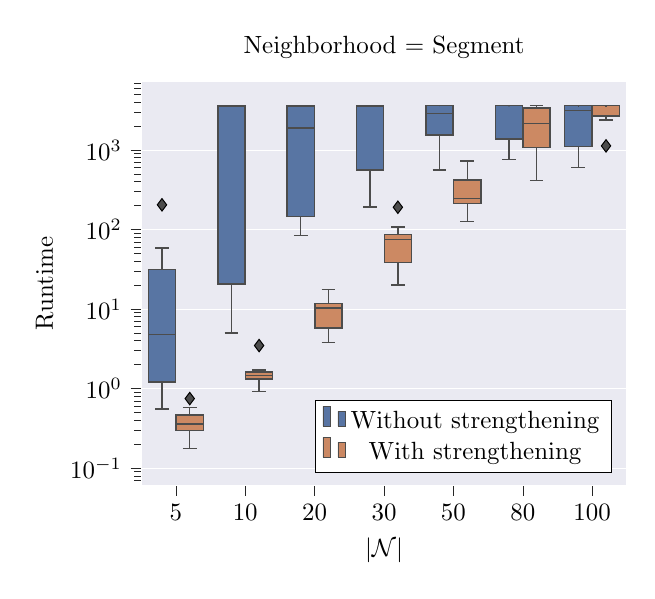
\begin{tikzpicture}[scale=0.9]
		
		\definecolor{color0}{rgb}{0.917647058823529,0.917647058823529,0.949019607843137}
		\definecolor{color1}{rgb}{0.347058823529412,0.458823529411765,0.641176470588235}
		\definecolor{color2}{rgb}{0.798529411764706,0.536764705882353,0.389705882352941}
		
		\begin{axis}[
			axis background/.style={fill=color0},
			axis line style={white},
			tick align=outside,
			title={Neighborhood = Segment},
			x grid style={white},
			xtick pos = left,
			ytick pos = left,
			xlabel={$|\mathcal N|$},
			% xmajorticks=false,
			xmin=-0.5, xmax=6.5,
			xtick style={color=white!15!black},
			xtick={0,1,2,3,4,5,6},
			xticklabels={5, 10, 20, 30, 50, 80, 100},
			y grid style={white},
			ylabel={Runtime},
			ymajorgrids,
			% ymajorticks=false,
			ymin=-0.05, ymax= 7200,
			log basis y={10},
			ymode = log,
			ytick style={color=white!15!black},
			%ytick={-0.2,0,0.2,0.4,0.6,0.8,1,1.2},
			%yticklabels={−0.2,0.0,0.2,0.4,0.6,0.8,1.0,1.2},
			legend pos = south east
			]
			\path [draw=white!29.8039215686275!black, fill=color1, semithick]
			(axis cs:-0.396,1.21752905845642)
			--(axis cs:-0.004,1.21752905845642)
			--(axis cs:-0.004,31.4301370382309)
			--(axis cs:-0.396,31.4301370382309)
			--(axis cs:-0.396,1.21752905845642)
			--cycle;
			\path [draw=white!29.8039215686275!black, fill=color2, semithick]
			(axis cs:0.004,0.298131942749023)
			--(axis cs:0.396,0.298131942749023)
			--(axis cs:0.396,0.465471982955933)
			--(axis cs:0.004,0.465471982955933)
			--(axis cs:0.004,0.298131942749023)
			--cycle;
			\path [draw=white!29.8039215686275!black, fill=color1, semithick]
			(axis cs:0.604,20.7727794647217)
			--(axis cs:0.996,20.7727794647217)
			--(axis cs:0.996,3600.03858071566)
			--(axis cs:0.604,3600.03858071566)
			--(axis cs:0.604,20.7727794647217)
			--cycle;
			\path [draw=white!29.8039215686275!black, fill=color2, semithick]
			(axis cs:1.004,1.31483119726181)
			--(axis cs:1.396,1.31483119726181)
			--(axis cs:1.396,1.61325573921204)
			--(axis cs:1.004,1.61325573921204)
			--(axis cs:1.004,1.31483119726181)
			--cycle;
			\path [draw=white!29.8039215686275!black, fill=color1, semithick]
			(axis cs:1.604,145.357283353806)
			--(axis cs:1.996,145.357283353806)
			--(axis cs:1.996,3600.26086455584)
			--(axis cs:1.604,3600.26086455584)
			--(axis cs:1.604,145.357283353806)
			--cycle;
			\path [draw=white!29.8039215686275!black, fill=color2, semithick]
			(axis cs:2.004,5.76829767227173)
			--(axis cs:2.396,5.76829767227173)
			--(axis cs:2.396,11.8237460255623)
			--(axis cs:2.004,11.8237460255623)
			--(axis cs:2.004,5.76829767227173)
			--cycle;
			\path [draw=white!29.8039215686275!black, fill=color1, semithick]
			(axis cs:2.604,559.95950448513)
			--(axis cs:2.996,559.95950448513)
			--(axis cs:2.996,3601.03108596802)
			--(axis cs:2.604,3601.03108596802)
			--(axis cs:2.604,559.95950448513)
			--cycle;
			\path [draw=white!29.8039215686275!black, fill=color2, semithick]
			(axis cs:3.004,38.516390144825)
			--(axis cs:3.396,38.516390144825)
			--(axis cs:3.396,87.1920122504234)
			--(axis cs:3.004,87.1920122504234)
			--(axis cs:3.004,38.516390144825)
			--cycle;
			\path [draw=white!29.8039215686275!black, fill=color1, semithick]
			(axis cs:3.604,1538.009141922)
			--(axis cs:3.996,1538.009141922)
			--(axis cs:3.996,3603.53307509422)
			--(axis cs:3.604,3603.53307509422)
			--(axis cs:3.604,1538.009141922)
			--cycle;
			\path [draw=white!29.8039215686275!black, fill=color2, semithick]
			(axis cs:4.004,211.856712222099)
			--(axis cs:4.396,211.856712222099)
			--(axis cs:4.396,418.142462968826)
			--(axis cs:4.004,418.142462968826)
			--(axis cs:4.004,211.856712222099)
			--cycle;
			\path [draw=white!29.8039215686275!black, fill=color1, semithick]
			(axis cs:4.604,1382.20820063353)
			--(axis cs:4.996,1382.20820063353)
			--(axis cs:4.996,3607.96597838402)
			--(axis cs:4.604,3607.96597838402)
			--(axis cs:4.604,1382.20820063353)
			--cycle;
			\path [draw=white!29.8039215686275!black, fill=color2, semithick]
			(axis cs:5.004,1069.18310433626)
			--(axis cs:5.396,1069.18310433626)
			--(axis cs:5.396,3399.26668268442)
			--(axis cs:5.004,3399.26668268442)
			--(axis cs:5.004,1069.18310433626)
			--cycle;
			\path [draw=white!29.8039215686275!black, fill=color1, semithick]
			(axis cs:5.604,1101.9550280571)
			--(axis cs:5.996,1101.9550280571)
			--(axis cs:5.996,3609.3919608593)
			--(axis cs:5.604,3609.3919608593)
			--(axis cs:5.604,1101.9550280571)
			--cycle;
			\path [draw=white!29.8039215686275!black, fill=color2, semithick]
			(axis cs:6.004,2693.49566185474)
			--(axis cs:6.396,2693.49566185474)
			--(axis cs:6.396,3615.86866497993)
			--(axis cs:6.004,3615.86866497993)
			--(axis cs:6.004,2693.49566185474)
			--cycle;
			\path [draw=white!29.8039215686275!black, fill=color1, semithick]
			(axis cs:6.604,3609.79030585289)
			--(axis cs:6.996,3609.79030585289)
			--(axis cs:6.996,3661.58016300201)
			--(axis cs:6.604,3661.58016300201)
			--(axis cs:6.604,3609.79030585289)
			--cycle;
			\path [draw=white!29.8039215686275!black, fill=color2, semithick]
			(axis cs:7.004,2998.95609879494)
			--(axis cs:7.396,2998.95609879494)
			--(axis cs:7.396,3618.01733189821)
			--(axis cs:7.004,3618.01733189821)
			--(axis cs:7.004,2998.95609879494)
			--cycle;
			\path [draw=white!29.8039215686275!black, fill=color1, semithick]
			(axis cs:7.604,1613.96234500408)
			--(axis cs:7.996,1613.96234500408)
			--(axis cs:7.996,3602.05603379011)
			--(axis cs:7.604,3602.05603379011)
			--(axis cs:7.604,1613.96234500408)
			--cycle;
			\path [draw=white!29.8039215686275!black, fill=color2, semithick]
			(axis cs:8.004,1789.22926878929)
			--(axis cs:8.396,1789.22926878929)
			--(axis cs:8.396,3610.1610725522)
			--(axis cs:8.004,3610.1610725522)
			--(axis cs:8.004,1789.22926878929)
			--cycle;
			\path [draw=white!29.8039215686275!black, fill=color1, semithick]
			(axis cs:8.604,3604.05633342266)
			--(axis cs:8.996,3604.05633342266)
			--(axis cs:8.996,3618.32394456863)
			--(axis cs:8.604,3618.32394456863)
			--(axis cs:8.604,3604.05633342266)
			--cycle;
			\path [draw=white!29.8039215686275!black, fill=color2, semithick]
			(axis cs:9.004,1851.82985758781)
			--(axis cs:9.396,1851.82985758781)
			--(axis cs:9.396,2931.76504272223)
			--(axis cs:9.004,2931.76504272223)
			--(axis cs:9.004,1851.82985758781)
			--cycle;
			\path [draw=white!29.8039215686275!black, fill=color1, semithick]
			(axis cs:9.604,3823.45712518692)
			--(axis cs:9.996,3823.45712518692)
			--(axis cs:9.996,3953.7330031395)
			--(axis cs:9.604,3953.7330031395)
			--(axis cs:9.604,3823.45712518692)
			--cycle;
			\path [draw=white!29.8039215686275!black, fill=color2, semithick]
			(axis cs:10.004,1628.18117189407)
			--(axis cs:10.396,1628.18117189407)
			--(axis cs:10.396,3111.13092088699)
			--(axis cs:10.004,3111.13092088699)
			--(axis cs:10.004,1628.18117189407)
			--cycle;
			\draw[draw=white!29.8039215686275!black,fill=color1,line width=0.3pt] (axis cs:0,0) rectangle (axis cs:0,0);
			\draw[draw=white!29.8039215686275!black,fill=color2,line width=0.3pt] (axis cs:0,0) rectangle (axis cs:0,0);
			\draw[draw=darkslategray76,fill=steelblue88116163,line width=0.3pt] (axis cs:0,0) rectangle (axis cs:0,0);
			\addlegendimage{ybar,ybar legend,draw=darkslategray76,fill=steelblue88116163,line width=0.3pt}
			\addlegendentry{Without strengthening}
			
			\draw[draw=darkslategray76,fill=peru20313699,line width=0.3pt] (axis cs:0,0) rectangle (axis cs:0,0);
			\addlegendimage{ybar,ybar legend,draw=darkslategray76,fill=peru20313699,line width=0.3pt}
			\addlegendentry{With strengthening}
			
			\addplot [semithick, white!29.8039215686275!black]
			table {%
				-0.2 1.21752905845642
				-0.2 0.55260705947876
			};
			\addplot [semithick, white!29.8039215686275!black]
			table {%
				-0.2 31.4301370382309
				-0.2 58.6506700515747
			};
			\addplot [semithick, white!29.8039215686275!black]
			table {%
				-0.298 0.55260705947876
				-0.102 0.55260705947876
			};
			\addplot [semithick, white!29.8039215686275!black]
			table {%
				-0.298 58.6506700515747
				-0.102 58.6506700515747
			};
			\addplot [black, mark=diamond*, mark size=2.5, mark options={solid,fill=white!29.8039215686275!black}, only marks]
			table {%
				-0.2 204.544420003891
			};
			\addplot [semithick, white!29.8039215686275!black]
			table {%
				0.2 0.298131942749023
				0.2 0.175446033477783
			};
			\addplot [semithick, white!29.8039215686275!black]
			table {%
				0.2 0.465471982955933
				0.2 0.575913906097412
			};
			\addplot [semithick, white!29.8039215686275!black]
			table {%
				0.102 0.175446033477783
				0.298 0.175446033477783
			};
			\addplot [semithick, white!29.8039215686275!black]
			table {%
				0.102 0.575913906097412
				0.298 0.575913906097412
			};
			\addplot [black, mark=diamond*, mark size=2.5, mark options={solid,fill=white!29.8039215686275!black}, only marks]
			table {%
				0.2 0.747928142547607
			};
			\addplot [semithick, white!29.8039215686275!black]
			table {%
				0.8 20.7727794647217
				0.8 4.96410608291626
			};
			\addplot [semithick, white!29.8039215686275!black]
			table {%
				0.8 3600.03858071566
				0.8 3600.14858388901
			};
			\addplot [semithick, white!29.8039215686275!black]
			table {%
				0.702 4.96410608291626
				0.898 4.96410608291626
			};
			\addplot [semithick, white!29.8039215686275!black]
			table {%
				0.702 3600.14858388901
				0.898 3600.14858388901
			};
			\addplot [semithick, white!29.8039215686275!black]
			table {%
				1.2 1.31483119726181
				1.2 0.921970129013062
			};
			\addplot [semithick, white!29.8039215686275!black]
			table {%
				1.2 1.61325573921204
				1.2 1.70817899703979
			};
			\addplot [semithick, white!29.8039215686275!black]
			table {%
				1.102 0.921970129013062
				1.298 0.921970129013062
			};
			\addplot [semithick, white!29.8039215686275!black]
			table {%
				1.102 1.70817899703979
				1.298 1.70817899703979
			};
			\addplot [black, mark=diamond*, mark size=2.5, mark options={solid,fill=white!29.8039215686275!black}, only marks]
			table {%
				1.2 3.47283411026001
			};
			\addplot [semithick, white!29.8039215686275!black]
			table {%
				1.8 145.357283353806
				1.8 83.976019859314
			};
			\addplot [semithick, white!29.8039215686275!black]
			table {%
				1.8 3600.26086455584
				1.8 3600.88121581078
			};
			\addplot [semithick, white!29.8039215686275!black]
			table {%
				1.702 83.976019859314
				1.898 83.976019859314
			};
			\addplot [semithick, white!29.8039215686275!black]
			table {%
				1.702 3600.88121581078
				1.898 3600.88121581078
			};
			\addplot [semithick, white!29.8039215686275!black]
			table {%
				2.2 5.76829767227173
				2.2 3.77168488502502
			};
			\addplot [semithick, white!29.8039215686275!black]
			table {%
				2.2 11.8237460255623
				2.2 17.7169480323792
			};
			\addplot [semithick, white!29.8039215686275!black]
			table {%
				2.102 3.77168488502502
				2.298 3.77168488502502
			};
			\addplot [semithick, white!29.8039215686275!black]
			table {%
				2.102 17.7169480323792
				2.298 17.7169480323792
			};
			\addplot [semithick, white!29.8039215686275!black]
			table {%
				2.8 559.95950448513
				2.8 192.698868989944
			};
			\addplot [semithick, white!29.8039215686275!black]
			table {%
				2.8 3601.03108596802
				2.8 3605.92868113518
			};
			\addplot [semithick, white!29.8039215686275!black]
			table {%
				2.702 192.698868989944
				2.898 192.698868989944
			};
			\addplot [semithick, white!29.8039215686275!black]
			table {%
				2.702 3605.92868113518
				2.898 3605.92868113518
			};
			\addplot [semithick, white!29.8039215686275!black]
			table {%
				3.2 38.516390144825
				3.2 20.0589971542358
			};
			\addplot [semithick, white!29.8039215686275!black]
			table {%
				3.2 87.1920122504234
				3.2 107.448718070984
			};
			\addplot [semithick, white!29.8039215686275!black]
			table {%
				3.102 20.0589971542358
				3.298 20.0589971542358
			};
			\addplot [semithick, white!29.8039215686275!black]
			table {%
				3.102 107.448718070984
				3.298 107.448718070984
			};
			\addplot [black, mark=diamond*, mark size=2.5, mark options={solid,fill=white!29.8039215686275!black}, only marks]
			table {%
				3.2 190.71932220459
			};
			\addplot [semithick, white!29.8039215686275!black]
			table {%
				3.8 1538.009141922
				3.8 561.059300899506
			};
			\addplot [semithick, white!29.8039215686275!black]
			table {%
				3.8 3603.53307509422
				3.8 3604.03469395638
			};
			\addplot [semithick, white!29.8039215686275!black]
			table {%
				3.702 561.059300899506
				3.898 561.059300899506
			};
			\addplot [semithick, white!29.8039215686275!black]
			table {%
				3.702 3604.03469395638
				3.898 3604.03469395638
			};
			\addplot [semithick, white!29.8039215686275!black]
			table {%
				4.2 211.856712222099
				4.2 125.601166963577
			};
			\addplot [semithick, white!29.8039215686275!black]
			table {%
				4.2 418.142462968826
				4.2 724.09502196312
			};
			\addplot [semithick, white!29.8039215686275!black]
			table {%
				4.102 125.601166963577
				4.298 125.601166963577
			};
			\addplot [semithick, white!29.8039215686275!black]
			table {%
				4.102 724.09502196312
				4.298 724.09502196312
			};
			\addplot [semithick, white!29.8039215686275!black]
			table {%
				4.8 1382.20820063353
				4.8 760.751152992249
			};
			\addplot [semithick, white!29.8039215686275!black]
			table {%
				4.8 3607.96597838402
				4.8 3608.99823284149
			};
			\addplot [semithick, white!29.8039215686275!black]
			table {%
				4.702 760.751152992249
				4.898 760.751152992249
			};
			\addplot [semithick, white!29.8039215686275!black]
			table {%
				4.702 3608.99823284149
				4.898 3608.99823284149
			};
			\addplot [semithick, white!29.8039215686275!black]
			table {%
				5.2 1069.18310433626
				5.2 413.9951608181
			};
			\addplot [semithick, white!29.8039215686275!black]
			table {%
				5.2 3399.26668268442
				5.2 3619.02899813652
			};
			\addplot [semithick, white!29.8039215686275!black]
			table {%
				5.102 413.9951608181
				5.298 413.9951608181
			};
			\addplot [semithick, white!29.8039215686275!black]
			table {%
				5.102 3619.02899813652
				5.298 3619.02899813652
			};
			\addplot [semithick, white!29.8039215686275!black]
			table {%
				5.8 1101.9550280571
				5.8 602.410846948624
			};
			\addplot [semithick, white!29.8039215686275!black]
			table {%
				5.8 3609.3919608593
				5.8 3611.7278239727
			};
			\addplot [semithick, white!29.8039215686275!black]
			table {%
				5.702 602.410846948624
				5.898 602.410846948624
			};
			\addplot [semithick, white!29.8039215686275!black]
			table {%
				5.702 3611.7278239727
				5.898 3611.7278239727
			};
			\addplot [semithick, white!29.8039215686275!black]
			table {%
				6.2 2693.49566185474
				6.2 2398.62307906151
			};
			\addplot [semithick, white!29.8039215686275!black]
			table {%
				6.2 3615.86866497993
				6.2 3622.43857002258
			};
			\addplot [semithick, white!29.8039215686275!black]
			table {%
				6.102 2398.62307906151
				6.298 2398.62307906151
			};
			\addplot [semithick, white!29.8039215686275!black]
			table {%
				6.102 3622.43857002258
				6.298 3622.43857002258
			};
			\addplot [black, mark=diamond*, mark size=2.5, mark options={solid,fill=white!29.8039215686275!black}, only marks]
			table {%
				6.2 1126.91467905045
			};
			\addplot [semithick, white!29.8039215686275!black]
			table {%
				6.8 3609.79030585289
				6.8 3609.79030585289
			};
			\addplot [semithick, white!29.8039215686275!black]
			table {%
				6.8 3661.58016300201
				6.8 3685.21105194092
			};
			\addplot [semithick, white!29.8039215686275!black]
			table {%
				6.702 3609.79030585289
				6.898 3609.79030585289
			};
			\addplot [semithick, white!29.8039215686275!black]
			table {%
				6.702 3685.21105194092
				6.898 3685.21105194092
			};
			\addplot [black, mark=diamond*, mark size=2.5, mark options={solid,fill=white!29.8039215686275!black}, only marks]
			table {%
				6.8 1402.30817294121
				6.8 1834.41865110397
			};
			\addplot [semithick, white!29.8039215686275!black]
			table {%
				7.2 2998.95609879494
				7.2 2438.48225498199
			};
			\addplot [semithick, white!29.8039215686275!black]
			table {%
				7.2 3618.01733189821
				7.2 3629.0251159668
			};
			\addplot [semithick, white!29.8039215686275!black]
			table {%
				7.102 2438.48225498199
				7.298 2438.48225498199
			};
			\addplot [semithick, white!29.8039215686275!black]
			table {%
				7.102 3629.0251159668
				7.298 3629.0251159668
			};
			\addplot [black, mark=diamond*, mark size=2.5, mark options={solid,fill=white!29.8039215686275!black}, only marks]
			table {%
				7.2 1536.34117817879
			};
			\addplot [semithick, white!29.8039215686275!black]
			table {%
				7.8 1613.96234500408
				7.8 804.753911972046
			};
			\addplot [semithick, white!29.8039215686275!black]
			table {%
				7.8 3602.05603379011
				7.8 3611.91618490219
			};
			\addplot [semithick, white!29.8039215686275!black]
			table {%
				7.702 804.753911972046
				7.898 804.753911972046
			};
			\addplot [semithick, white!29.8039215686275!black]
			table {%
				7.702 3611.91618490219
				7.898 3611.91618490219
			};
			\addplot [semithick, white!29.8039215686275!black]
			table {%
				8.2 1789.22926878929
				8.2 1641.86067605019
			};
			\addplot [semithick, white!29.8039215686275!black]
			table {%
				8.2 3610.1610725522
				8.2 3634.07880687714
			};
			\addplot [semithick, white!29.8039215686275!black]
			table {%
				8.102 1641.86067605019
				8.298 1641.86067605019
			};
			\addplot [semithick, white!29.8039215686275!black]
			table {%
				8.102 3634.07880687714
				8.298 3634.07880687714
			};
			\addplot [semithick, white!29.8039215686275!black]
			table {%
				8.8 3604.05633342266
				8.8 3602.16263890266
			};
			\addplot [semithick, white!29.8039215686275!black]
			table {%
				8.8 3618.32394456863
				8.8 3619.19555306435
			};
			\addplot [semithick, white!29.8039215686275!black]
			table {%
				8.702 3602.16263890266
				8.898 3602.16263890266
			};
			\addplot [semithick, white!29.8039215686275!black]
			table {%
				8.702 3619.19555306435
				8.898 3619.19555306435
			};
			\addplot [black, mark=diamond*, mark size=2.5, mark options={solid,fill=white!29.8039215686275!black}, only marks]
			table {%
				8.8 2760.11033797264
				8.8 3750.57215499878
			};
			\addplot [semithick, white!29.8039215686275!black]
			table {%
				9.2 1851.82985758781
				9.2 516.475353002548
			};
			\addplot [semithick, white!29.8039215686275!black]
			table {%
				9.2 2931.76504272223
				9.2 3645.80811190605
			};
			\addplot [semithick, white!29.8039215686275!black]
			table {%
				9.102 516.475353002548
				9.298 516.475353002548
			};
			\addplot [semithick, white!29.8039215686275!black]
			table {%
				9.102 3645.80811190605
				9.298 3645.80811190605
			};
			\addplot [semithick, white!29.8039215686275!black]
			table {%
				9.8 3823.45712518692
				9.8 3644.2532851696
			};
			\addplot [semithick, white!29.8039215686275!black]
			table {%
				9.8 3953.7330031395
				9.8 3970.15586400032
			};
			\addplot [semithick, white!29.8039215686275!black]
			table {%
				9.702 3644.2532851696
				9.898 3644.2532851696
			};
			\addplot [semithick, white!29.8039215686275!black]
			table {%
				9.702 3970.15586400032
				9.898 3970.15586400032
			};
			\addplot [semithick, white!29.8039215686275!black]
			table {%
				10.2 1628.18117189407
				10.2 952.006986856461
			};
			\addplot [semithick, white!29.8039215686275!black]
			table {%
				10.2 3111.13092088699
				10.2 3608.51588511467
			};
			\addplot [semithick, white!29.8039215686275!black]
			table {%
				10.102 952.006986856461
				10.298 952.006986856461
			};
			\addplot [semithick, white!29.8039215686275!black]
			table {%
				10.102 3608.51588511467
				10.298 3608.51588511467
			};
			\addplot [semithick, white!29.8039215686275!black]
			table {%
				-0.396 4.79820585250854
				-0.004 4.79820585250854
			};
			\addplot [semithick, white!29.8039215686275!black]
			table {%
				0.004 0.357388019561768
				0.396 0.357388019561768
			};
			\addplot [semithick, white!29.8039215686275!black]
			table {%
				0.604 3600.02458703518
				0.996 3600.02458703518
			};
			\addplot [semithick, white!29.8039215686275!black]
			table {%
				1.004 1.4667774438858
				1.396 1.4667774438858
			};
			\addplot [semithick, white!29.8039215686275!black]
			table {%
				1.604 1900.91373944283
				1.996 1900.91373944283
			};
			\addplot [semithick, white!29.8039215686275!black]
			table {%
				2.004 10.307445526123
				2.396 10.307445526123
			};
			\addplot [semithick, white!29.8039215686275!black]
			table {%
				2.604 3600.8377289772
				2.996 3600.8377289772
			};
			\addplot [semithick, white!29.8039215686275!black]
			table {%
				3.004 75.2547216415405
				3.396 75.2547216415405
			};
			\addplot [semithick, white!29.8039215686275!black]
			table {%
				3.604 2885.36510300636
				3.996 2885.36510300636
			};
			\addplot [semithick, white!29.8039215686275!black]
			table {%
				4.004 246.94141793251
				4.396 246.94141793251
			};
			\addplot [semithick, white!29.8039215686275!black]
			table {%
				4.604 3605.92392551899
				4.996 3605.92392551899
			};
			\addplot [semithick, white!29.8039215686275!black]
			table {%
				5.004 2142.84770703316
				5.396 2142.84770703316
			};
			\addplot [semithick, white!29.8039215686275!black]
			table {%
				5.604 3119.12695789337
				5.996 3119.12695789337
			};
			\addplot [semithick, white!29.8039215686275!black]
			table {%
				6.004 3605.78131246567
				6.396 3605.78131246567
			};
			\addplot [semithick, white!29.8039215686275!black]
			table {%
				6.604 3612.72732686996
				6.996 3612.72732686996
			};
			\addplot [semithick, white!29.8039215686275!black]
			table {%
				7.004 3606.13559997082
				7.396 3606.13559997082
			};
			\addplot [semithick, white!29.8039215686275!black]
			table {%
				7.604 2757.28104102612
				7.996 2757.28104102612
			};
			\addplot [semithick, white!29.8039215686275!black]
			table {%
				8.004 3605.36972546577
				8.396 3605.36972546577
			};
			\addplot [semithick, white!29.8039215686275!black]
			table {%
				8.604 3612.72326803207
				8.996 3612.72326803207
			};
			\addplot [semithick, white!29.8039215686275!black]
			table {%
				9.004 2072.36165392399
				9.396 2072.36165392399
			};
			\addplot [semithick, white!29.8039215686275!black]
			table {%
				9.604 3899.30706095695
				9.996 3899.30706095695
			};
			\addplot [semithick, white!29.8039215686275!black]
			table {%
				10.004 2151.40807795525
				10.396 2151.40807795525
			};
		\end{axis}
		
	\end{tikzpicture}
	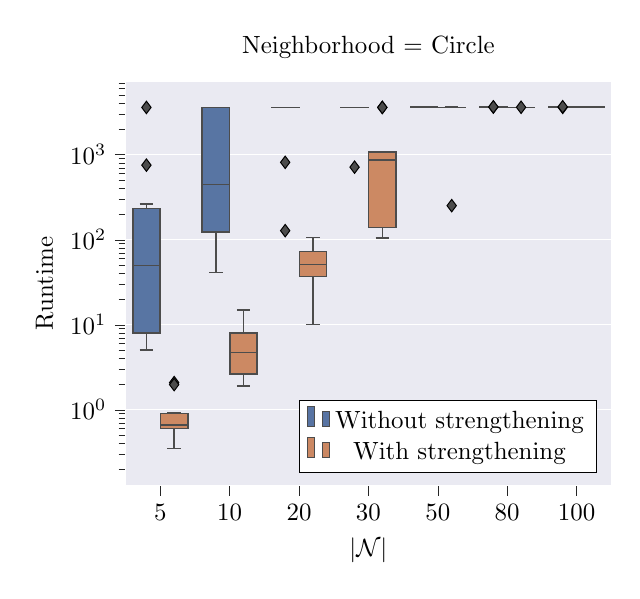
\begin{tikzpicture}[scale=0.9]

	\definecolor{color0}{rgb}{0.917647058823529,0.917647058823529,0.949019607843137}
	\definecolor{color1}{rgb}{0.347058823529412,0.458823529411765,0.641176470588235}
	\definecolor{color2}{rgb}{0.798529411764706,0.536764705882353,0.389705882352941}
	
\begin{axis}[
	axis background/.style={fill=color0},
	axis line style={white},
	tick align=outside,
	title={Neighborhood = Circle},
	x grid style={white},
	xtick pos = left,
	ytick pos = left,
	xlabel={$|\mathcal N|$},
	% xmajorticks=false,
	xmin=-0.5, xmax=6.5,
	xtick style={color=white!15!black},
	xtick={0,1,2,3,4,5,6},
	xticklabels={5, 10, 20, 30, 50, 80, 100},
	y grid style={white},
	ylabel={Runtime},
	ymajorgrids,
	% ymajorticks=false,
	ymin=-0.05, ymax= 7200,
	log basis y={10},
	ymode = log,
	ytick style={color=white!15!black},
	%ytick={-0.2,0,0.2,0.4,0.6,0.8,1,1.2},
	%yticklabels={−0.2,0.0,0.2,0.4,0.6,0.8,1.0,1.2},
	legend pos = south east
	]
	\path [draw=white!29.8039215686275!black, fill=color1, semithick]
	(axis cs:-0.396,8.05090779066086)
	--(axis cs:-0.004,8.05090779066086)
	--(axis cs:-0.004,231.816551744938)
	--(axis cs:-0.396,231.816551744938)
	--(axis cs:-0.396,8.05090779066086)
	--cycle;
	\path [draw=white!29.8039215686275!black, fill=color2, semithick]
	(axis cs:0.004,0.603522717952728)
	--(axis cs:0.396,0.603522717952728)
	--(axis cs:0.396,0.908215522766113)
	--(axis cs:0.004,0.908215522766113)
	--(axis cs:0.004,0.603522717952728)
	--cycle;
	\path [draw=white!29.8039215686275!black, fill=color1, semithick]
	(axis cs:0.604,124.218014419079)
	--(axis cs:0.996,124.218014419079)
	--(axis cs:0.996,3600.13461649418)
	--(axis cs:0.604,3600.13461649418)
	--(axis cs:0.604,124.218014419079)
	--cycle;
	\path [draw=white!29.8039215686275!black, fill=color2, semithick]
	(axis cs:1.004,2.65239107608795)
	--(axis cs:1.396,2.65239107608795)
	--(axis cs:1.396,7.98592978715897)
	--(axis cs:1.004,7.98592978715897)
	--(axis cs:1.004,2.65239107608795)
	--cycle;
	\path [draw=white!29.8039215686275!black, fill=color1, semithick]
	(axis cs:1.604,3600.32590913773)
	--(axis cs:1.996,3600.32590913773)
	--(axis cs:1.996,3600.98365181684)
	--(axis cs:1.604,3600.98365181684)
	--(axis cs:1.604,3600.32590913773)
	--cycle;
	\path [draw=white!29.8039215686275!black, fill=color2, semithick]
	(axis cs:2.004,36.9325481057167)
	--(axis cs:2.396,36.9325481057167)
	--(axis cs:2.396,73.0904644727707)
	--(axis cs:2.004,73.0904644727707)
	--(axis cs:2.004,36.9325481057167)
	--cycle;
	\path [draw=white!29.8039215686275!black, fill=color1, semithick]
	(axis cs:2.604,3600.95979499817)
	--(axis cs:2.996,3600.95979499817)
	--(axis cs:2.996,3605.23400402069)
	--(axis cs:2.604,3605.23400402069)
	--(axis cs:2.604,3600.95979499817)
	--cycle;
	\path [draw=white!29.8039215686275!black, fill=color2, semithick]
	(axis cs:3.004,139.045187950134)
	--(axis cs:3.396,139.045187950134)
	--(axis cs:3.396,1071.0302670002)
	--(axis cs:3.004,1071.0302670002)
	--(axis cs:3.004,139.045187950134)
	--cycle;
	\path [draw=white!29.8039215686275!black, fill=color1, semithick]
	(axis cs:3.604,3603.63751798868)
	--(axis cs:3.996,3603.63751798868)
	--(axis cs:3.996,3627.92520177364)
	--(axis cs:3.604,3627.92520177364)
	--(axis cs:3.604,3603.63751798868)
	--cycle;
	\path [draw=white!29.8039215686275!black, fill=color2, semithick]
	(axis cs:4.004,3601.75783377886)
	--(axis cs:4.396,3601.75783377886)
	--(axis cs:4.396,3610.75702470541)
	--(axis cs:4.004,3610.75702470541)
	--(axis cs:4.004,3601.75783377886)
	--cycle;
	\path [draw=white!29.8039215686275!black, fill=color1, semithick]
	(axis cs:4.604,3645.77219605446)
	--(axis cs:4.996,3645.77219605446)
	--(axis cs:4.996,3647.84180998802)
	--(axis cs:4.604,3647.84180998802)
	--(axis cs:4.604,3645.77219605446)
	--cycle;
	\path [draw=white!29.8039215686275!black, fill=color2, semithick]
	(axis cs:5.004,3602.54204702377)
	--(axis cs:5.396,3602.54204702377)
	--(axis cs:5.396,3607.71199470758)
	--(axis cs:5.004,3607.71199470758)
	--(axis cs:5.004,3602.54204702377)
	--cycle;
	\path [draw=white!29.8039215686275!black, fill=color1, semithick]
	(axis cs:5.604,3650.0892868042)
	--(axis cs:5.996,3650.0892868042)
	--(axis cs:5.996,3655.93269896507)
	--(axis cs:5.604,3655.93269896507)
	--(axis cs:5.604,3650.0892868042)
	--cycle;
	\path [draw=white!29.8039215686275!black, fill=color2, semithick]
	(axis cs:6.004,3612.44972205162)
	--(axis cs:6.396,3612.44972205162)
	--(axis cs:6.396,3620.63622152805)
	--(axis cs:6.004,3620.63622152805)
	--(axis cs:6.004,3612.44972205162)
	--cycle;
	\path [draw=white!29.8039215686275!black, fill=color1, semithick]
	(axis cs:6.604,3611.01951909065)
	--(axis cs:6.996,3611.01951909065)
	--(axis cs:6.996,3682.25671100617)
	--(axis cs:6.604,3682.25671100617)
	--(axis cs:6.604,3611.01951909065)
	--cycle;
	\path [draw=white!29.8039215686275!black, fill=color2, semithick]
	(axis cs:7.004,3602.27094990015)
	--(axis cs:7.396,3602.27094990015)
	--(axis cs:7.396,3620.05129808187)
	--(axis cs:7.004,3620.05129808187)
	--(axis cs:7.004,3602.27094990015)
	--cycle;
	\path [draw=white!29.8039215686275!black, fill=color1, semithick]
	(axis cs:7.604,3614.71244698763)
	--(axis cs:7.996,3614.71244698763)
	--(axis cs:7.996,3619.78759926558)
	--(axis cs:7.604,3619.78759926558)
	--(axis cs:7.604,3614.71244698763)
	--cycle;
	\path [draw=white!29.8039215686275!black, fill=color2, semithick]
	(axis cs:8.004,3606.27544140816)
	--(axis cs:8.396,3606.27544140816)
	--(axis cs:8.396,3618.18070554733)
	--(axis cs:8.004,3618.18070554733)
	--(axis cs:8.004,3606.27544140816)
	--cycle;
	\draw[draw=white!29.8039215686275!black,fill=color1,line width=0.3pt] (axis cs:0,0) rectangle (axis cs:0,0);
	\draw[draw=darkslategray76,fill=steelblue88116163,line width=0.3pt] (axis cs:0,0) rectangle (axis cs:0,0);
	\addlegendimage{ybar,ybar legend,draw=darkslategray76,fill=steelblue88116163,line width=0.3pt}
	\addlegendentry{Without strengthening}
	
	\draw[draw=darkslategray76,fill=peru20313699,line width=0.3pt] (axis cs:0,0) rectangle (axis cs:0,0);
	\addlegendimage{ybar,ybar legend,draw=darkslategray76,fill=peru20313699,line width=0.3pt}
	\addlegendentry{With strengthening}
	
	\addplot [semithick, white!29.8039215686275!black]
	table {%
	-0.2 8.05090779066086
	-0.2 5.07074117660522
	};
	\addplot [semithick, white!29.8039215686275!black]
	table {%
	-0.2 231.816551744938
	-0.2 263.470886945724
	};
	\addplot [semithick, white!29.8039215686275!black]
	table {%
	-0.298 5.07074117660522
	-0.102 5.07074117660522
	};
	\addplot [semithick, white!29.8039215686275!black]
	table {%
	-0.298 263.470886945724
	-0.102 263.470886945724
	};
	\addplot [black, mark=diamond*, mark size=2.5, mark options={solid,fill=white!29.8039215686275!black}, only marks]
	table {%
	-0.2 754.546452045441
	-0.2 3600.01791596413
	};
	\addplot [semithick, white!29.8039215686275!black]
	table {%
	0.2 0.603522717952728
	0.2 0.349291086196899
	};
	\addplot [semithick, white!29.8039215686275!black]
	table {%
	0.2 0.908215522766113
	0.2 0.926176071166992
	};
	\addplot [semithick, white!29.8039215686275!black]
	table {%
	0.102 0.349291086196899
	0.298 0.349291086196899
	};
	\addplot [semithick, white!29.8039215686275!black]
	table {%
	0.102 0.926176071166992
	0.298 0.926176071166992
	};
	\addplot [black, mark=diamond*, mark size=2.5, mark options={solid,fill=white!29.8039215686275!black}, only marks]
	table {%
	0.2 2.09010004997253
	0.2 1.97804403305054
	};
	\addplot [semithick, white!29.8039215686275!black]
	table {%
	0.8 124.218014419079
	0.8 41.4265987873077
	};
	\addplot [semithick, white!29.8039215686275!black]
	table {%
	0.8 3600.13461649418
	0.8 3600.64154601097
	};
	\addplot [semithick, white!29.8039215686275!black]
	table {%
	0.702 41.4265987873077
	0.898 41.4265987873077
	};
	\addplot [semithick, white!29.8039215686275!black]
	table {%
	0.702 3600.64154601097
	0.898 3600.64154601097
	};
	\addplot [semithick, white!29.8039215686275!black]
	table {%
	1.2 2.65239107608795
	1.2 1.90428996086121
	};
	\addplot [semithick, white!29.8039215686275!black]
	table {%
	1.2 7.98592978715897
	1.2 14.8280959129333
	};
	\addplot [semithick, white!29.8039215686275!black]
	table {%
	1.102 1.90428996086121
	1.298 1.90428996086121
	};
	\addplot [semithick, white!29.8039215686275!black]
	table {%
	1.102 14.8280959129333
	1.298 14.8280959129333
	};
	\addplot [semithick, white!29.8039215686275!black]
	table {%
	1.8 3600.32590913773
	1.8 3600.3246421814
	};
	\addplot [semithick, white!29.8039215686275!black]
	table {%
	1.8 3600.98365181684
	1.8 3601.79518413544
	};
	\addplot [semithick, white!29.8039215686275!black]
	table {%
	1.702 3600.3246421814
	1.898 3600.3246421814
	};
	\addplot [semithick, white!29.8039215686275!black]
	table {%
	1.702 3601.79518413544
	1.898 3601.79518413544
	};
	\addplot [black, mark=diamond*, mark size=2.5, mark options={solid,fill=white!29.8039215686275!black}, only marks]
	table {%
	1.8 814.182178974152
	1.8 128.000700950623
	};
	\addplot [semithick, white!29.8039215686275!black]
	table {%
	2.2 36.9325481057167
	2.2 10.123596906662
	};
	\addplot [semithick, white!29.8039215686275!black]
	table {%
	2.2 73.0904644727707
	2.2 106.525239944458
	};
	\addplot [semithick, white!29.8039215686275!black]
	table {%
	2.102 10.123596906662
	2.298 10.123596906662
	};
	\addplot [semithick, white!29.8039215686275!black]
	table {%
	2.102 106.525239944458
	2.298 106.525239944458
	};
	\addplot [semithick, white!29.8039215686275!black]
	table {%
	2.8 3600.95979499817
	2.8 3600.86448287964
	};
	\addplot [semithick, white!29.8039215686275!black]
	table {%
	2.8 3605.23400402069
	2.8 3606.08144116402
	};
	\addplot [semithick, white!29.8039215686275!black]
	table {%
	2.702 3600.86448287964
	2.898 3600.86448287964
	};
	\addplot [semithick, white!29.8039215686275!black]
	table {%
	2.702 3606.08144116402
	2.898 3606.08144116402
	};
	\addplot [black, mark=diamond*, mark size=2.5, mark options={solid,fill=white!29.8039215686275!black}, only marks]
	table {%
	2.8 714.146538972855
	};
	\addplot [semithick, white!29.8039215686275!black]
	table {%
	3.2 139.045187950134
	3.2 105.201857089996
	};
	\addplot [semithick, white!29.8039215686275!black]
	table {%
	3.2 1071.0302670002
	3.2 1071.0302670002
	};
	\addplot [semithick, white!29.8039215686275!black]
	table {%
	3.102 105.201857089996
	3.298 105.201857089996
	};
	\addplot [semithick, white!29.8039215686275!black]
	table {%
	3.102 1071.0302670002
	3.298 1071.0302670002
	};
	\addplot [black, mark=diamond*, mark size=2.5, mark options={solid,fill=white!29.8039215686275!black}, only marks]
	table {%
	3.2 3600.56792497635
	3.2 3600.48221802711
	};
	\addplot [semithick, white!29.8039215686275!black]
	table {%
	3.8 3603.63751798868
	3.8 3603.40955495834
	};
	\addplot [semithick, white!29.8039215686275!black]
	table {%
	3.8 3627.92520177364
	3.8 3635.57329106331
	};
	\addplot [semithick, white!29.8039215686275!black]
	table {%
	3.702 3603.40955495834
	3.898 3603.40955495834
	};
	\addplot [semithick, white!29.8039215686275!black]
	table {%
	3.702 3635.57329106331
	3.898 3635.57329106331
	};
	\addplot [semithick, white!29.8039215686275!black]
	table {%
	4.2 3601.75783377886
	4.2 3601.16748690605
	};
	\addplot [semithick, white!29.8039215686275!black]
	table {%
	4.2 3610.75702470541
	4.2 3619.59864997864
	};
	\addplot [semithick, white!29.8039215686275!black]
	table {%
	4.102 3601.16748690605
	4.298 3601.16748690605
	};
	\addplot [semithick, white!29.8039215686275!black]
	table {%
	4.102 3619.59864997864
	4.298 3619.59864997864
	};
	\addplot [black, mark=diamond*, mark size=2.5, mark options={solid,fill=white!29.8039215686275!black}, only marks]
	table {%
	4.2 252.03409910202
	};
	\addplot [semithick, white!29.8039215686275!black]
	table {%
	4.8 3645.77219605446
	4.8 3645.77219605446
	};
	\addplot [semithick, white!29.8039215686275!black]
	table {%
	4.8 3647.84180998802
	4.8 3647.84180998802
	};
	\addplot [semithick, white!29.8039215686275!black]
	table {%
	4.702 3645.77219605446
	4.898 3645.77219605446
	};
	\addplot [semithick, white!29.8039215686275!black]
	table {%
	4.702 3647.84180998802
	4.898 3647.84180998802
	};
	\addplot [black, mark=diamond*, mark size=2.5, mark options={solid,fill=white!29.8039215686275!black}, only marks]
	table {%
	4.8 3638.69181895256
	4.8 3655.34494805336
	};
	\addplot [semithick, white!29.8039215686275!black]
	table {%
	5.2 3602.54204702377
	5.2 3601.95828700066
	};
	\addplot [semithick, white!29.8039215686275!black]
	table {%
	5.2 3607.71199470758
	5.2 3614.88623595238
	};
	\addplot [semithick, white!29.8039215686275!black]
	table {%
	5.102 3601.95828700066
	5.298 3601.95828700066
	};
	\addplot [semithick, white!29.8039215686275!black]
	table {%
	5.102 3614.88623595238
	5.298 3614.88623595238
	};
	\addplot [black, mark=diamond*, mark size=2.5, mark options={solid,fill=white!29.8039215686275!black}, only marks]
	table {%
	5.2 3618.48321509361
	};
	\addplot [semithick, white!29.8039215686275!black]
	table {%
	5.8 3650.0892868042
	5.8 3650.0892868042
	};
	\addplot [semithick, white!29.8039215686275!black]
	table {%
	5.8 3655.93269896507
	5.8 3655.93269896507
	};
	\addplot [semithick, white!29.8039215686275!black]
	table {%
	5.702 3650.0892868042
	5.898 3650.0892868042
	};
	\addplot [semithick, white!29.8039215686275!black]
	table {%
	5.702 3655.93269896507
	5.898 3655.93269896507
	};
	\addplot [black, mark=diamond*, mark size=2.5, mark options={solid,fill=white!29.8039215686275!black}, only marks]
	table {%
	5.8 3609.60879087448
	5.8 3666.14317202568
	};
	\addplot [semithick, white!29.8039215686275!black]
	table {%
	6.2 3612.44972205162
	6.2 3605.29008984566
	};
	\addplot [semithick, white!29.8039215686275!black]
	table {%
	6.2 3620.63622152805
	6.2 3622.51985788345
	};
	\addplot [semithick, white!29.8039215686275!black]
	table {%
	6.102 3605.29008984566
	6.298 3605.29008984566
	};
	\addplot [semithick, white!29.8039215686275!black]
	table {%
	6.102 3622.51985788345
	6.298 3622.51985788345
	};
	\addplot [semithick, white!29.8039215686275!black]
	table {%
	6.8 3611.01951909065
	6.8 3605.90529203415
	};
	\addplot [semithick, white!29.8039215686275!black]
	table {%
	6.8 3682.25671100617
	6.8 3709.81486797333
	};
	\addplot [semithick, white!29.8039215686275!black]
	table {%
	6.702 3605.90529203415
	6.898 3605.90529203415
	};
	\addplot [semithick, white!29.8039215686275!black]
	table {%
	6.702 3709.81486797333
	6.898 3709.81486797333
	};
	\addplot [semithick, white!29.8039215686275!black]
	table {%
	7.2 3602.27094990015
	7.2 3600.73966503143
	};
	\addplot [semithick, white!29.8039215686275!black]
	table {%
	7.2 3620.05129808187
	7.2 3633.49116778374
	};
	\addplot [semithick, white!29.8039215686275!black]
	table {%
	7.102 3600.73966503143
	7.298 3600.73966503143
	};
	\addplot [semithick, white!29.8039215686275!black]
	table {%
	7.102 3633.49116778374
	7.298 3633.49116778374
	};
	\addplot [semithick, white!29.8039215686275!black]
	table {%
	7.8 3614.71244698763
	7.8 3609.47614216805
	};
	\addplot [semithick, white!29.8039215686275!black]
	table {%
	7.8 3619.78759926558
	7.8 3620.59529304504
	};
	\addplot [semithick, white!29.8039215686275!black]
	table {%
	7.702 3609.47614216805
	7.898 3609.47614216805
	};
	\addplot [semithick, white!29.8039215686275!black]
	table {%
	7.702 3620.59529304504
	7.898 3620.59529304504
	};
	\addplot [semithick, white!29.8039215686275!black]
	table {%
	8.2 3606.27544140816
	8.2 3604.48313188553
	};
	\addplot [semithick, white!29.8039215686275!black]
	table {%
	8.2 3618.18070554733
	8.2 3628.29366016388
	};
	\addplot [semithick, white!29.8039215686275!black]
	table {%
	8.102 3604.48313188553
	8.298 3604.48313188553
	};
	\addplot [semithick, white!29.8039215686275!black]
	table {%
	8.102 3628.29366016388
	8.298 3628.29366016388
	};
	\addplot [semithick, white!29.8039215686275!black]
	table {%
	-0.396 49.783145070076
	-0.004 49.783145070076
	};
	\addplot [semithick, white!29.8039215686275!black]
	table {%
	0.004 0.659420967102051
	0.396 0.659420967102051
	};
	\addplot [semithick, white!29.8039215686275!black]
	table {%
	0.604 446.667264938354
	0.996 446.667264938354
	};
	\addplot [semithick, white!29.8039215686275!black]
	table {%
	1.004 4.71278297901154
	1.396 4.71278297901154
	};
	\addplot [semithick, white!29.8039215686275!black]
	table {%
	1.604 3600.39011096954
	1.996 3600.39011096954
	};
	\addplot [semithick, white!29.8039215686275!black]
	table {%
	2.004 50.9535143375397
	2.396 50.9535143375397
	};
	\addplot [semithick, white!29.8039215686275!black]
	table {%
	2.604 3601.32289600372
	2.996 3601.32289600372
	};
	\addplot [semithick, white!29.8039215686275!black]
	table {%
	3.004 861.480319976807
	3.396 861.480319976807
	};
	\addplot [semithick, white!29.8039215686275!black]
	table {%
	3.604 3626.84971487522
	3.996 3626.84971487522
	};
	\addplot [semithick, white!29.8039215686275!black]
	table {%
	4.004 3602.61586940289
	4.396 3602.61586940289
	};
	\addplot [semithick, white!29.8039215686275!black]
	table {%
	4.604 3645.98594808578
	4.996 3645.98594808578
	};
	\addplot [semithick, white!29.8039215686275!black]
	table {%
	5.004 3604.91833150387
	5.396 3604.91833150387
	};
	\addplot [semithick, white!29.8039215686275!black]
	table {%
	5.604 3652.72786307335
	5.996 3652.72786307335
	};
	\addplot [semithick, white!29.8039215686275!black]
	table {%
	6.004 3619.63726186752
	6.396 3619.63726186752
	};
	\addplot [semithick, white!29.8039215686275!black]
	table {%
	6.604 3665.61946201324
	6.996 3665.61946201324
	};
	\addplot [semithick, white!29.8039215686275!black]
	table {%
	7.004 3604.44044959545
	7.396 3604.44044959545
	};
	\addplot [semithick, white!29.8039215686275!black]
	table {%
	7.604 3617.98812496662
	7.996 3617.98812496662
	};
	\addplot [semithick, white!29.8039215686275!black]
	table {%
	8.004 3608.06775093079
	8.396 3608.06775093079
	};
\end{axis}
\end{tikzpicture}

\caption{Runtime of the model \eqref{form:H-TSPN} without and with preprocessing when the neighborhoods are segments and balls.}
\label{fig:Fig4}
\end{figure}